\xchapter{Avaliação da disponibilidade dos softwares científicos}
{Este capítulo apresenta a caracterização dos softwares científicos de análise
estática de código-fonte quanto à sua disponibilidade de código-fonte.}
\label{caracterizacao-ferramentas}

%Caracterizar os {\it softwares científicos} do domínio de aplicação de análise
%estática de código-fonte publicados em conferências de engenharia de software
%com objetivo de compreender como estão sendo publicados e mantidos, com
%especial atenção à disponibilidade de seu código-fonte.

Muitos estudos em engenharia de software sofrem de dificuldades de repetição
\cite{Tang2016}, uma prática importante para aumentar a validade científica dos
estudos e seus resultados. {\it Repetição} é a atividade de refazer exatamente
o que outra pessoa fez usando os artefatos originais, a disponibilidade de
código-fonte é o requisito mínimo para possibilitar tal prática.

Avaliar as publicações da área de engenharia de software e identificar como
publicam código-fonte dos softwares desenvolvidos é importante para sabermos o
quão possível é repetir tais estudos, uma prática necessária para verificar a
validade e aumentar o nível de confiança do seus resultados, além de ser
importantes para a divulgação do conhecimento empregado em tais softwares.

A subárea da engenharia de software dedicada a pesquisas sobre análise estática
de código-fonte tem uma longa e respeitável tradição, e apesar da constante
evolução da área e do surgimento frequente de softwares de análise de
código-fonte, existe ainda uma carência de estudos avaliando tais softwares
\cite{Li2010}, especialmente os {\it softwares científicos}.

Tradicionalmente os autores de {\it software científico} enfrentam problemas
com a disponibilidade de tais softwares \cite{Prlic2012}, avaliar o quanto este
problema ocorre na subárea de análise estática de código-fonte se mostra
útil como forma de diagnosticar o quanto a área preocupa-se em resolver ou
solucionar tal questão.

Assim temos como objetivo geral deste estudo avaliar e caracterizar a
disponibilidade dos softwares cientificos de análise estática de código-fonte
publicados em conferências de engenharia de software.

%A busca por {\it softwares científicos} será limitado pelo domínio de aplicação
%de análise estática de código-fonte, visto que esta área possui carência de estudos
%avaliando suas ferramentas, desta forma conseguimos contribuir com a área de
%análise estática de código-fonte ao mesmo tempo que exploramos o quanto os
%pesquisadores publicando softwares nesta área publicam e disponibilizam seus
%softwares e desta forma contribuem para divulgação dos resultados e proporcionam
%repetição dos estudos.

\section{Planejamento do estudo}

% * Introduction
% * Background
% * Experimental Setup (hipoteses / design)
% * Results (data analysis)
% * Discussion
% * Threats to validity
% * Conclusions
% 
% # Scope [why?]
% ## Goal
% # Planning [how?]
% ## Context selection
% ## Hypothesis Formulation
% ## Variables selection
% ## Selection of subjects
% ## Experiment design
% ### Choice of experiment design
% ### General design principles
% ### Standard design types
% ## Instrumentation
% ## Validity evaluation
% # Operation
% # Analysis and Interpretation
% ## Teste de hipótese
%
%\section{Data collection procedure}
%
%\begin{itemize}
%  \item Revisão estruturada para busca e seleção de ferramentas a partir de artigos acadêmicos
%  \item Caracterização inicial das ferramentas, dimensões: Linguagem, Lançamentos
%  \item Caracterização final das ferramentas, dimensões: Entrada, Linguagens suportadas
%\end{itemize}

\subsection{Seleção de softwares científicos}

A seleção de softwares científicos será realizado através de uma {\it revisão
estruturada}, um processo disciplinado para busca e seleção de {\it softwares
científicos} de um domínio específico a partir de critérios bem definidos, de
forma que seja possível a reprodução do estudo por parte de pesquisadores
interessados.

A revisão estruturada difere da revisão e do mapeamento sistemático por ser um
processo mais simples e menos rígido, onde o resultado final é um conjunto de
softwares, enquanto no mapeamento ou na revisão sistemática há um esforço em
caracterizar os artigos analisados o mesmo não ocorre na revisão estruturada.

A revisão estruturada é organizada em três atividades de (1) busca de artigos
(definição das fontes, obtenção dos artigos nas fontes), (2) filtro (definição
de critérios de busca, definição de script de busca) e (3) seleção de artigos
com publicação de softwares. Estas atividades estão representadas na Figura
\ref{figura-revisao-estruturada}.

\begin{figure}[h]
  \center
  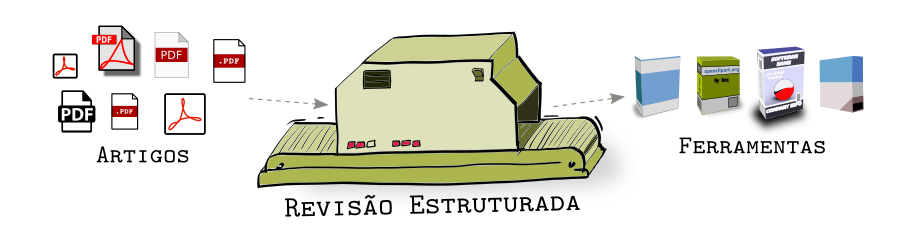
\includegraphics[scale=0.21]{imagens/revisao-estruturada.png}
  \caption{Atividades da revisão estruturada: (1) busca, (2) filtro e (3) seleção}
  \label{figura-revisao-estruturada}
\end{figure}

Na primeira atividade da revisão estruturada são definidas as fontes de busca,
estas fontes são conferências que abordam o tema de interesse do estudo, e que
apresentam um grande potencial de encontrar softwares do domínio de aplicação
desejado. Esta primeira atividade de busca deve incluir o maior número possível
de ediçoes das conferências selecionadas, para cada edição são copiados
localmente todos os artigos em PDF para posterior filtro nas atividades
subsequentes.

A segunda atividade da revisão estruturada realizada em cima de todo o conjunto
de artigos é um filtro automática que busca em todo o conteúdo dos artigos os
termos de interesse, estes termos devem ser pensados em relaçao ao domínio de
aplicação desejado, devem ser abrangentes a fim de evitar falsos negativos.
Os seguintes termos serão utilizados nesta atividade de filtro:

\begin{verbatim}
  "tool" OU "framework"; E
  "download" OU "available"; E
  "http" OU "ftp"; E
  "static analysis" OU "parser".
\end{verbatim}

Estes termos devem encontrar artigos com publicação de {\it softwares
científicos} do domínio de análise estática de código-fonte com disponibilidade
para {\it download}, seja binário ou código-fonte.

A terceira e última atividade da revisão estruturada é a seleção de artigos,
nela é identificado se cada artigo resulta, de fato, em publicação de {\it
software científico} do domínio de aplicação desejado. Esta seleção é feita a
partir de uma leitura superficial do artigo em busca de indícios de que o
artigo publica um software do domínio em questão.

Nesta etapa cada artigo é lido, inicialmente apenas introdução, resultados e
conclusão com o objetivo de identificar se o artigo publica {\it software
científico} e indica onde obter uma cópia do software. {\it Softwares
científicos} que sejam mais abrangentes do que apenas análise estática de
código-fonte mas que contenham esta função em seu conjunto também são
selecionadas.

\subsection{Avaliação da disponibilidade dos softwares científicos}

Os {\it softwares científicos} de análise estática de código-fonte selecionados
na revisão estruturada serão avaliados em relação à sua disponibilidade visto a
importância de tais artefatos para a divulgação do conhecimento e para
replicação dos resultados das pesquisas em engenharia de software.

Dois aspectos serão levados em conta nesta avaliação, um relacionado à como o
artigo apresenta o {\it software científico} em relação à sua disponibilidade e
o outro relacionado a como o software está de fato disponível, se a fonte
informada está funcional ou não. O primeiro aspecto é o seguinte:

\begin{description}

  \item {\it Disponibilidade - como o artigo disponibiliza o software científico:}
    \begin{itemize}
      \item Artigo não indica onde obter o software\\
        {\it \small artigo não indica fonte para obtenção do software}
      \item Fonte para obtenção do software indisponível\\
        {\it \small artigo indica fonte mas encontra-se inacessível, fora do ar ou com erros}
      \item Software disponivel, binários ou código-fonte\\
        {\it \small a fonte indicada está disponível e acessível}
    \end{itemize}

\end{description}

Este primeiro aspecto tem importancia de mostrar quantos artigos falham em
não informar ao leitor fontes para obtenção de tais artefatos, mesmo que por
eventura o autor tenha disponibilizado o código-fonte dos artefatos produzidos,
o fato de não informarem a fonte inviabiliza, ou ao menos dificulta, bastante
pesquisadores interessados em repetir ou reproduzir os resultados de tais estudos.

A fonte indicada será testada a fim de identificar se ainda estão disponíveis e
se é possível obter uma cópia do software em tal fonte, links para download
serão testados e documentados de acordo seu estado, se estão funcionando, se
estão indisponíveis, etc.

Em seguida os softwares disponíveis, aqueles caracterizados como ``Software
disponivel, binários ou código-fonte'' serão caracterizados com detalhes sobre
sua disponibilidade, se tem código-fonte disponível e usam licença de software
livre ou código aberto.

Para isto tomaremos como base o trabalho de \citeonline{Novak2010}, neste
estudo o autor propôe uma taxonomia e um conjunto de dimensões para
caracterização de ferramentas de análise estática. Iremos utilizar a categoria
relacionada à disponibilidade dos softwares.

\begin{description}

  \item {\it Disponibilidade - de que forma a ferramenta está disponível:}
    \begin{itemize}
      \item Código Aberto ({\it Open Source})\\
        {\it \small a ferramenta é livre e o código-fonte está disponível}
      \item Grátis ({\it Free})\\
        {\it \small a ferramenta é grátis mas o código-fonte não está disponível}
      \item Comercial\\
        {\it \small a ferramenta está disponível mediante pagamento}
    \end{itemize}

\end{description}

Este aspecto está relacionado ao estado do software em relação à
disponibilidade do código-fonte, será feito o download do software e avaliado
a disponibilidade de código-fonte e qual licença o author da ferramenta
usa. Vale lembrar que apenas os artigos que oferecem fonte disponíveis, ou seja,
links ainda funcionando para obtenção e download da ferramenta, serão considerados
na caracterização deste segundo aspecto.

Este segundo aspecto enfatiza como o código-fonte está disponível, se é livre,
se usa ou não alguma licença. A disponibilidade do código-fonte, mesmo quando
não se usa licenças livres, tem fudamental importância pois permite
pesquisadores interessados em estudar o conhecimento empregado ali, bem como,
repetir e reproduzir os resultados do estudo original.

A fonte de informação para essa caracterização segundo estas duas categorias
serão os artigos relacionados aos softwares, o código-fonte, documentos e site
do projeto. A disponibilidade dos {\it softwares científicos} como {\it código
aberto} representa o caso ideal, mesmo quando o autor não especifica uma
licença iremos considerar como código aberto, mesmo não sendo, esta decisão de
englobar como código aberto mesmo os que não citam licença é por conta da
importância na disponibilidade do software e de seu código-fonte, mesmo quando
o autor explicitamente não põe uma licença livre dando direitos para modificar
o código-fonte ao menos a disponibilidade permite que o código seja estudado e
isto já é suficiente para repetir ou replicar um dado estudo.

\section{Resultados}

Para a {\it revisão estruturada} foi selecionada a conferência SCAM - {\it
Source Code Analysis and Manipulation Working
Conference}\footnote{http://www.ieee-scam.org} e a conferência ASE - {\it
Automated Software Engineering}\footnote{http://ase-conferences.org}, por serem
ambas conferências com largo histórico de publicação sobre análise de
programas.

A primeira atividade da revisão estruturada -- {\it (2) Busca} -- passa por todas as ediçoes
destas duas conferências até o ano de 2015, uma lista completa e o endereço de
cada edição onde os artigos foram obtidos está documentado no Apêndice
\ref{edicoes-conferencias}, lá é indicado o endereço da conferência nos
respectivos portais onde os artigos em PDF foram obtidos.

Esta atividade de busca resultou num total de 1879 artigos, 346 artigos do SCAM
e 1533 artigos do ASE, a Figura \ref{grafico-total-artigos} (a) apresenta um
gráfico com estes números.

\begin{figure}[H]
  \center
  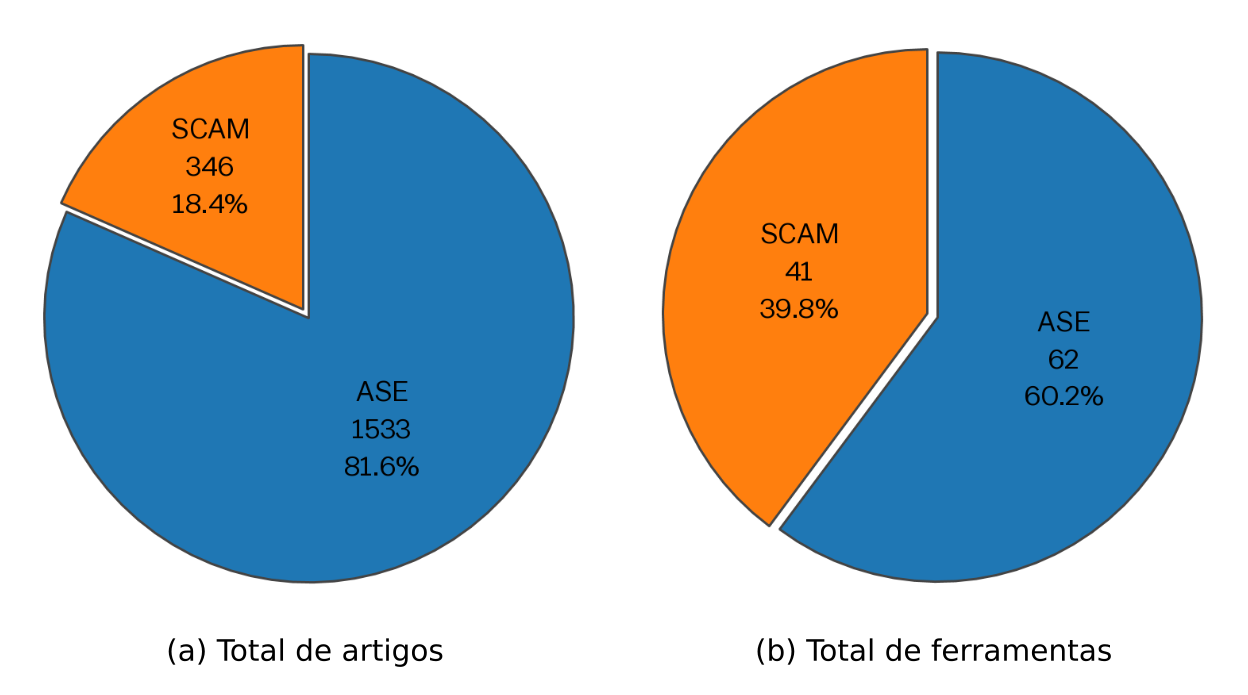
\includegraphics[scale=0.9]{imagens/total-artigos-e-ferramentas.png}
  \caption{Total de artigos e ferramentas por conferência (até o ano de 2015)}
  \label{grafico-total-artigos}
\end{figure}

A segunda atividade da revisão estruturada -- {\it (2) Filtro} -- realizado nesta
etapa no conjunto de 1879 artigos resultou em 436 artigos,
155 artigos da conferência SCAM e 281 da conferência ASE.

Estes 436 artigos com possível publicação de {\it software científico} de
análise estática de código-fonte contém em seu conteúdo os seguintes termos
utilizados no filtro automático.

\begin{verbatim}
  "tool" OU "framework"; E
  "download" OU "available"; E
  "http" OU "ftp"; E
  "static analysis" OU "parser".
\end{verbatim}

A última atividade da revisão estruturada -- (3) Seleção -- resultou em 103
artigos com publicação de {\it software científico} do domínio de aplicação de
análise estática de código-fonte, deste total 41 são da conferência
SCAM e 62 da conferência ASE, a Figura \ref{grafico-total-artigos} (b) e as
Figuras \ref{ferramentas-por-conferencia} (a) e (b) apresentam um resumo destes
números, as Tabelas \ref{artigos-do-scam} e \ref{artigos-do-ase} detalham os
resultados da revisão para cada edição das conferências analisadas.

\begin{figure}[h]
  \center
  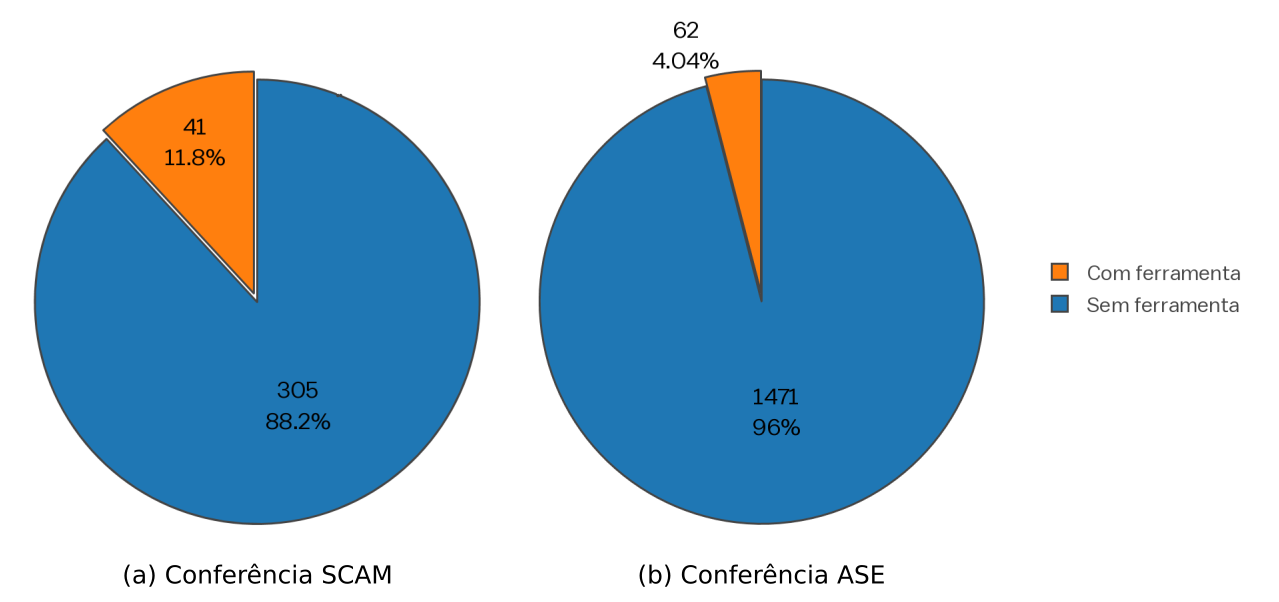
\includegraphics[scale=1]{imagens/ferramentas-por-conferencia.png}
  \caption{Total de artigos com ferramentas (até o ano de 2015)}
  \label{ferramentas-por-conferencia}
\end{figure}

Dos 346 artigos do SCAM analisados na revisão estruturada 44\% (155 artigos)
continham os termos pesquisados no filtro automático da segunda atividade de
revisão e 11\% (41 artigos) foram selecionados na terceira e última atividade
da revisão contendo publicação de ferramenta de análise estática.

Dos 1533 artigos do ASE analisados na revisão estruturada 18\% (281 artigos)
continham os termos pesquisados no filtro automático da segunda atividade de
revisão e apenas 4\% (62 artigos) foram selecionados na terceira e última
atividade da revisão contendo publicação de ferramenta de análise estática.

\begin{figure}[h]
  \center
  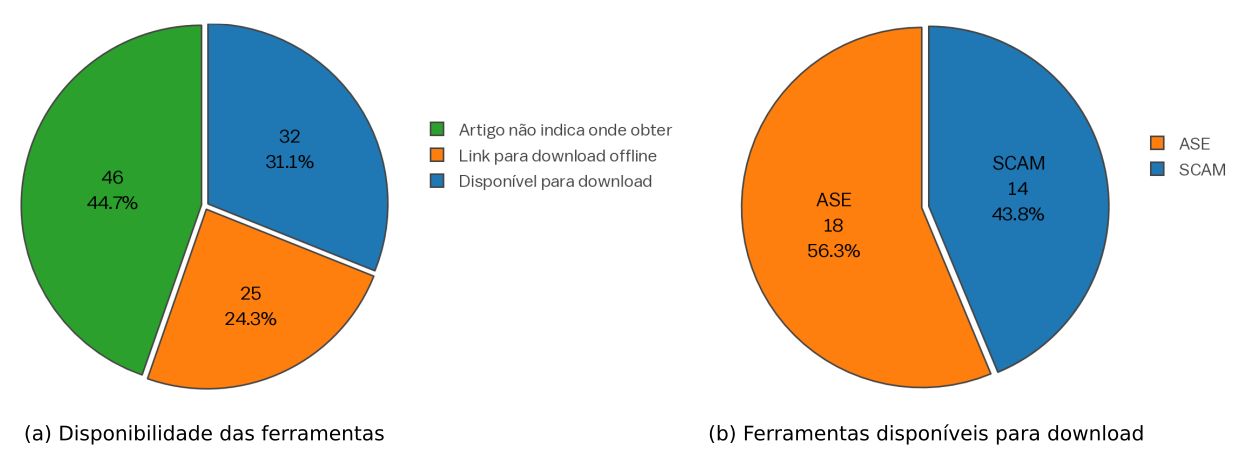
\includegraphics[scale=0.85]{imagens/ferramentas-disponiveis.png}
  \caption{Ferramentas disponíveis para download (até o ano de 2015)}
  \label{ferramentas-disponiveis}
\end{figure}

As informações foram obtidas de forma manual lendo o artigo onde a ferramenta foi publicada,
uma lista com todas as ferramentas selecionadas em ambas as conferências e sua descrição
é apresentada no Apendice \ref{softwares-cientificos}.

Esta avaliação da disponibilidade dos softwares científicos foi realizada num
conjunto de 35 softwares, estes foi o resultado da avaliação do primeiro
aspecto.  Total de 35 softwares científicos disponível para download, deste
conjunto, 32 são de código aberto e 3 são grátis (apenas binários disponíveis).

\section{Ameaças à validade}

...

\section{Conclusões}

Encontramos 103 artigos com publicação de {\it software científico} de análise
estática de código-fonte, apenas 35 possuem fonte para obtenção do software,
sendo 32 de código aberto, ou seja, com disponibilidade de código-fonte, e 3
grátis, apenas binários disponível. Ou seja, apenas 31\% dos artigos com
publicação de software disponibilizam o código-fonte das mesmas. Isto significa
que 69\% dos artigos são potencialmente impossíveis de serem repetidos, já que
os artefatos originais são necessários para tal atividade.

% analise e interpretação

% documentar onde os dados, fontes, etc podem ser encontrados:

% os artigos foram documentados e estão disponíveis num arquivo externo
% {\it artigos.ods}\footnote{http://github.com/joenio/dissertacao-ufba-2016/blob/master/revisao-estruturada/artigos.ods}.
%
%com o auxílio do script
%{\it
%filter}\footnote{http://github.com/joenio/dissertacao-ufba-2016/blob/master/revisao-estruturada/filter}
%escrito especialmente para este estudo. 
%
%atividade (2) da revisao estruturada:
%Os artigos selecionados nesta atividade
%estão documentados no arquivo {\it artigos.ods} indicados na coluna ``Filtro(2)''
%quando for o caso.
%
%A Tabela
%\ref{total-de-ferramentas} resume este total trazendo o nome de cada ferramenta
%e algumas de suas características, a caracterização completa está documentado
%no arquivo {\it
%ferramentas-e-metricas.ods}\footnote{https://github.com/joenio/dissertacao-ufba-2016/blob/master/dataset/ferramentas-e-metricas.ods}
%disponível no repositório desta dissertação.
